\section{Discovering Equivalent Programs}
\label{bg:sec:discovering_equivalent_programs}

In this section, we explain existing optimization methods to restructure
numerical programs with arithmetic equivalences.  Because general numerical
programs---consisting of program statements, conditional branches and
loops---supersede arithmetic expressions, we start by introducing optimization
methods of expressions, followed by those of general numerical programs.


\subsection{Improving Performance by Rewriting Arithmetic Expressions}
\label{bg:sub:performance}

\subsubsection{Software Compilers}

It is common knowledge to software programmers that a typical optimizing
compiler, such as GCC~\cite{gcc} and Clang~\cite{clang}, has some traditional
static analysis-based optimization passes such as dead code elimination, loop
strength reduction and constant propagation.  These optimization passes,
however, limit themselves by producing implementations that do not impact
numerical accuracy, \ie~they compute the same output given identical inputs.

A less well-known fact about these compilers is that they also support a
variety of optimization passes that are not enabled by default.  These options,
when enabled, allow the compiler to yield faster software implementations for
programs with a large proportion of floating-point arithmetic computations.
These optimization passes rewrite arithmetic expressions into more efficient
alternative forms which are equivalent to the originals in real arithmetic,
but when executed on a machine they compute different results.  The reason
for the differences is that arithmetic in machines has finite precision,
computed results must be rounded to the nearest representable values.  These
discrepancies, when accumulated, could potentially result in wildly inaccurate
outputs.

There are a number of compiler options in GCC~\cite{gcc} that specifically
performs the above optimizations.  For example, the following options exist to
enable expression-rewriting heuristics:
\begin{itemize}

    \item \verb|-fassociative-math| enables arithmetic expression rewriting by
    associativity, one of the heuristics applied is to perform exponentiation
    by squaring, \eg~an expression \verb|x*x*x*x| which requires 3
    multiplications, can be optimized as \verb|(x*x)*(x*x)|, reducing the
    number of multiplications to 2 by sharing the value of the subexpression
    \verb|x*x|;

    \item \verb|-freciprocal-math| can be used to rewrite $x / y$ into $x * (1
    / y)$, if $1 / y$ can be commonly shared among subexpressions; and

    \item \verb|-fno-signed-zeros| ignores the signedness of floating point
    zeros, for example, \verb|0.0f| and \verb|-0.0f| are identical, so that
    \verb|0.0f*x| can be simplified to \verb|0.0| without concerning us with
    the signedness of the result.

\end{itemize}

An additional optimization option, which encompasses the above options,
can be used to enable them all together; it further highlights
the \emph{unsafe} nature of these transformations in its name,
\ie~\verb|-funsafe-math-optimizations|.  Besides GCC, Clang, which uses the
LLVM framework, provides a similar option, \verb|-enable-unsafe-fp-math| to use
arithmetic equivalences to reduce the number of floating-point operations in a
program, by possibly sacrificing numerical accuracy.

% To give an example, the value $\sqrt{2}$, being irrational, can not be
% represented exactly in single-precision floating point, and thus must be
% rounded.

\subsubsection{High-Level Synthesis Tools}

In addition to the unsafe arithmetic expression rewriting heuristics inherited
from the LLVM framework, Vivado HLS~\cite{vivado_hls} and LegUp~\cite{legup},
which are both LLVM-based, can make use of hardware-specific optimization
passes to allow greater parallelism in synthesized circuit, thus improving
throughput.  The newly designed transformation to allow data-flow graphs to be
restructured to improve loop parallelism, which allows more computation across
loop iterations to overlap, and subsequently faster programs.  Xilinx's Vivado
HLS has a similar feature called \emph{expression balancing}~\cite{vivado_hls},
which aims to balance an arithmetic expression tree using associativity.  Tree
height reduction~\cite{nicolau91} further incorporates distributivity and
control-flow rewriting.  However, neither of these methods produces optimal
loop pipelining, as they do not examine the implications of loop-carried
dependences.  For example, a loop body:
\begin{lstlisting}
    sum = ((sum + A[i]) + B[i]) + C[i];
\end{lstlisting}\vspace{-15pt}
when synthesized in Vivado HLS with expression balancing, will produce a
schedule which corresponds to the following:
\begin{lstlisting}
    sum = (sum + A[i]) + (B[i] + C[i]);
\end{lstlisting}\vspace{-15pt}
This loop is more efficient than the original, because it has a delay of $2$
adders between consecutive iterations, instead of the original $3$-adder delay,
in the inter-iteration dependences of \verb|sum|.  However, as we will see
below, there is still room for improvement.

Canis~\etal~\cite{canis14} propose a similar approach called \emph{recurrence
minimization}.  They specifically tackle loop pipelining by incrementally
restructuring dependence graphs to minimize longest paths of recurrences.
Their method is subsequently incorporated in LegUp~\cite{legup}.  For instance,
by synthesizing the same original loop in LegUp, it detects that there are
inter-iteration dependences between each pair of \verb|sum| from consecutive
iterations.  The tool will therefore minimize the latency between these
dependences by using associativity to restructure the expression.  This
optimization produces a schedule which corresponds to the following loop body:
\begin{lstlisting}
    sum = sum + ((A[i] + B[i]) + C[i]);
\end{lstlisting}\vspace{-15pt}
It is notable that, by further delaying the addition of \verb|sum|, the loop
now has only a delay of $1$ adder between consecutive iterations.  This
technique can greatly reduce the run time of pipelined loops, especially if the
inter-iteration dependences has a long chain of additions.  However, similar to
Vivado HLS, they only apply associativity in their restructuring.

\subsubsection{Polynomial Factorization}

The above mentioned tools restrict themselves to simple arithmetic
equivalences, as they are intended for fast and simple optimizations that
can easily be applied by a compiler.  A further handful of techniques take
one step further, by focusing on multivariate polynomials, and factorizing
them to minimize the number of arithmetic operations in an expression.  These
approaches are applicable to both software and hardware designs, as they
minimize the number of operations in an expression, the throughput of the
optimized design can be reduced.  In addition, in an FPGA circuit, this will
also translate to a reduction of resources utilized.

It is well known that the Horner scheme is the optimal way to
factorize a univariate polynomial so that its operator count is
minimized~\cite{neumaier01}, \eg~a polynomial $x^3 + 2x^2 + 3x + 4$,
which uses 4 multipliers and 3 adders if common subexpressions are
eliminated, can be factorized into $x(x(x + 2) + 3) + 4$, which uses 2
fewer multipliers.  However, a multivariate polynomial could be expressed
in multiple ways using the Horner scheme, and finding the optimal one is
a difficult problem.  Ceberio~\etal~\cite{ceberio04} therefore propose a
greedy algorithm to efficiently factorize a multivariate polynomial to
overcome this.  Hosangadi~\etal~\cite{hosangadi} propose an algorithm for the
factorization of polynomials, in order to eliminate common subexpressions, and
subsequently reduce addition and multiplication counts for a faster software
implementation.  However it is not possible to choose different optimization
levels with their method.  Peymandoust~\etal~\cite{peymandoust} present an
approach that only deals with the factorization of polynomials in HLS using
\groebner~bases.  The weaknesses of this are its dependence on a set of
library expressions~\cite{hosangadi} and the high computational complexity of
\groebner~bases.

\subsubsection{Shortcomings}

The above approaches utilize a number of heuristics to rewrite expressions, and
do not explore all possible rewrites in full by taking into account additional
equivalence relations.  This could limit their applicability to a small number
of special cases.  The implementation obtained therefore is often likely
to be suboptimal, as further improvements are possible.  More importantly,
none of the above mentioned techniques and tools aim to minimize, or even
analyze, the impact of their transformations on numerical accuracy.  HLS tools
therefore generally disable these unsafe features by default for floating-point
computations.  It is in general a good practice to avoid them, if numerical
accuracy is a critical factor to ensure the correctness of the application
being compiled.

% Later we will discuss techniques that can reason about and optimize numerical
% accuracy in programs.

\subsection{Rewriting Arithmetic Expressions for Accuracy}
\label{bg:sub:expression_accuracy}

In many numerically sensitive programs, small round-off errors, when
accumulated, would result in catastrophically inaccurate results.  In
particular, Panchekha~\etal~\cite{panchekha15} show that inaccurate
computations, due to round-off errors, resulted in the retraction of scientific
articles~\cite{altman99}, and even wild discrepancies in stock market
indices~\cite{mccullough99}.  In response, the software community has seen an
emergence of techniques that rewrites expressions in numerical programs, to
ameliorate round-off errors in numerically sensitive applications.  However,
round-off errors in numerical programs are well known to be perplexing to
debug~\cite{toronto14}, and it is in general difficult to apply intuitions
manually and rewrite programs to optimize numerical accuracy~\cite{toronto14}.
The numerical accuracy optimization techniques therefore often explore the
search space of equivalent expressions, using equivalence relations in
real arithmetic, ranging from the simplest possible, \eg~associativity,
commutativity and distributivity, to more sophisticated ones, such as
trigonometry facts, rules derived from heuristics $x - y = \frac{x^2 - y^2}{x
+ y}$~\cite{panchekha15}, and many more.

As the vastness of the search space prohibits us to explore it fully, authors
confronting this problem resolve to heuristics.  Darulova~\etal~\cite{darulova}
use genetic programming to evolve the structure of arithmetic expressions
into more accurate forms.  However there are several disadvantages with
metaheuristics, such as convergence can only be proved empirically and
scalability is difficult to control because there is no definitive method to
decide how long the algorithm must run until it reaches a satisfactory goal.
The method proposed by Martel~\cite{martel07} is based on operational semantics
with abstract interpretation, but even their depth limited strategy is, in
practice, at least exponentially complex.  Ioualalen~\etal~\cite{ioualalen},
create a polynomial-size structure, APEG, to represent an exponential number of
equivalent expressions related by rules of equivalence.  However it restricts
itself to only a handful of these rules to avoid combinatorial explosion
of the structure and offers no options for tuning its optimization level.
Panchekha~\etal~\cite{panchekha15} present a tool, Herbie, which employs a
greedy hill-climbing heuristic to iteratively rewrite expressions in locations
that introduce the largest round-off errors.  Here, detailed overviews are
provided for two distinct approaches, APEG and Herbie.

\subsubsection{APEG}

The APEG proposed by Ioualalen~\etal~\cite{ioualalen} was inspired by E-PEG,
originally introduced by Tate~\etal~\cite{tate09}\footnote{E-PEG and equality
saturation is discussed in Section~\ref{bg:sub:equality_saturation}}.
E-PEGs, originally intended to discover equivalent structure in programs
but not arithmetic expressions, nevertheless include equivalence rules
that are similar to the ones that exist in real arithmetic.  For instance,
distributivity can by applied over nodes such as $\theta$ and $\mathrm{eval}$
nodes.

The APEG is similar in construction to the E-PEG, which is also a graph-based
structure, and promotes the maximal sharing of common subtrees.  The major
difference is that because of the lack of control-flow in the program, APEGs
are acyclic, and do not consist of nodes that correspond to control-flows.
APEGs supersede arithmetic expression by allowing all possible nodes in an
arithmetic expression, \ie~it can contain leaf nodes such as a constant
value or a variable identifier, unary or binary arithmetic operators that
respectively have one or two child nodes.  In addition, to allow an APEG to
encode exponential number of equivalent expressions within a polynomial space,
it further introduces two different kinds of nodes that efficiently model
equivalences.

Firstly, the APEG defines a node that contains an \emph{abstraction box},
\fbox{$\opsymbol, \left(p_1, p_2, \mathellipsis, p_n\right)$}\,, where
$\opsymbol$ is a commutative associative operator such as addition $+$ and
multiplication $\times$, and $p_1, p_2, \mathellipsis, p_n$ are the children of
this node.  The abstraction box can be used to represent equivalent expressions
generated by different associative parsings of the expression $p_1 \opsymbol
p_2 \opsymbol \mathellipsis \opsymbol p_n$.  To illustrate, an expression $a
+ b + c$ can be encoded by the abstraction box \fbox{$+, (a, b, c)$}\,, which
can represent all equivalent parsings of the original expression, \ie~$(a
+ b) + c$, $a + (b + c)$ and $(a + c) + b$.  Each abstraction box with $n$
children can represent up to $(2n - 3){!!}$ equivalent expressions without
commutativity~\cite{ioualalen, mouilleron}, as commutativity do not impact
numerical accuracy for commutative operators.

Secondly, in an analogous fashion to the E-PEG, the APEG additionally
admits a new kind of nodes which can be used to enclose a set of equivalent
subexpressions.  Defined as $\langle p_1, p_2, \mathellipsis, p_n \rangle$,
the \emph{equivalent class} is a node which signifies all children subtrees
with root nodes $p_1, p_2, \mathellipsis, p_n$ represent expressions that are
mathematically equivalent.  This is analogous to forming equivalence edges in
E-PEGs.

\begin{figure}[ht]
    \centering
    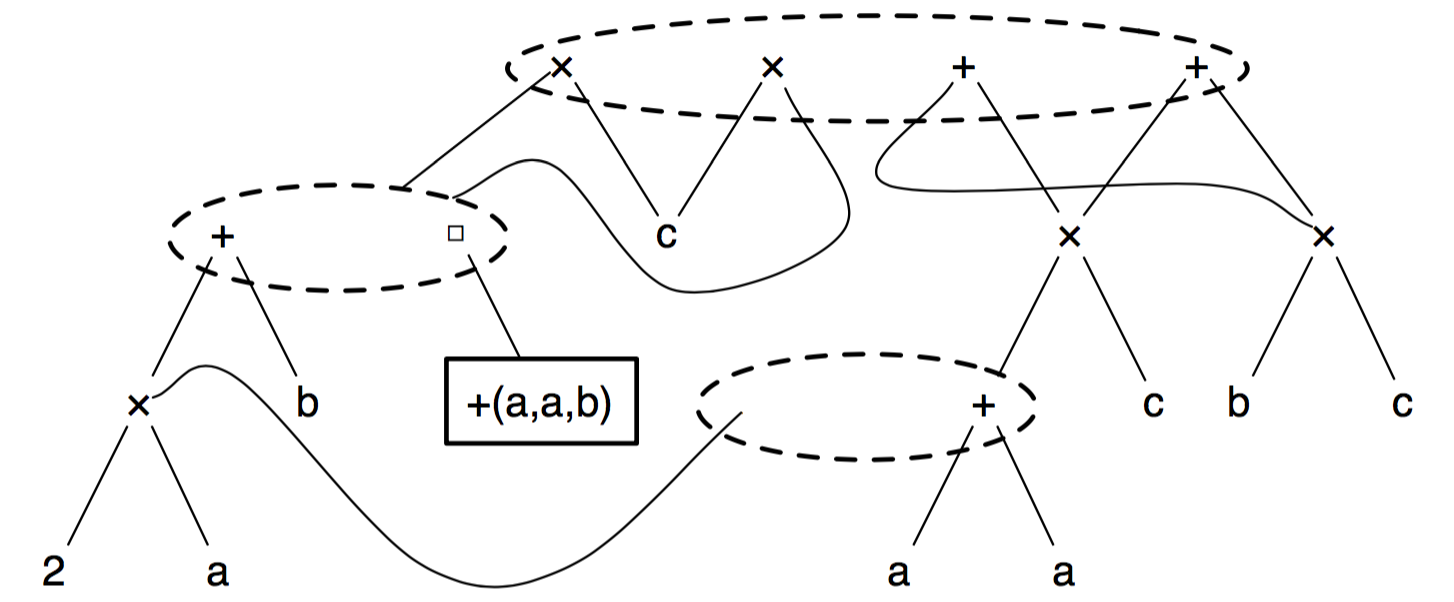
\includegraphics[scale=0.4]{bg/fig/apeg.png}
    \caption{%
        An example APEG for the expression $\left( \left( a + a \right) + b
        \right)$, taken from~\cite{martel12}.}\label{bg:fig:apeg}
\end{figure}
Take Figure~\ref{bg:fig:apeg} as our example, which not only contains standard
tree nodes which we would expect from an arithmetic expression tree, but
also an abstraction box and equivalent classes.  Each equivalent class is
represented by an ellipse with a dashed border.  It is evident that each
equivalent class indeed reflect a set of equivalent subtrees.  For instance,
consider the bottom equivalent class which has two equivalent subtrees, the
left and right ones represent $2 \times a$ and $a + a$ respectively.  Moreover,
as the subexpression $(a + a) + b$ is a summation of multiple elements, an
abstraction box \fbox{$+, (a, a, b)$}\, can therefore model the equivalent
parsings of it.

Despite the compactness of APEGs, searching for the most accurate expression
within an APEG is still exponentially complex.  For instance, consider an APEG
with $n$ equivalent classes, each contains $2$ different choices, in the worst
case, this may amount to a search of $2^n$ distinct equivalent expressions, so
as to determine the optimal solution.  To resolve this problem, the authors
of~\cite{ioualalen} employs a depth-limited search heuristic to reduce the size
of the search space.\footnote{The exact technique is not explained in their
original contribution.}  Additionally, as it was explained earlier, the time
complexity to search for the optimal parsing of an abstraction box is double
factorial.  They hence make use of another heuristic, which greedily pairs up
terms in an abstraction box $B = \text{\fbox{$+, \left(p_1, p_2, \mathellipsis,
p_n\right)$}}$\,.  To begin, the method searches for a pair of child subtrees
$p_i$ and $p_j$ in $B$, such that the expression $p_i \opsymbol p_j$ computes
with the smallest round-off error.  The nodes $p_i$ and $p_j$ are subsequently
removed from $B$, and a new subtree
\tikz[baseline=-2.3ex]{%
    \newcommand{\edgelength}{3.6ex}
    \node(op) at (0, 0) {\small $\opsymbol$};
    \node(pi) at (-\edgelength, -\edgelength) {\small $p_i$};
    \node(pj) at (\edgelength, -\edgelength) {\small $p_j$};
    \draw(op)--(pi);
    \draw(op)--(pj);
}
is then added to $B$.  The above procedure is then iteratively repeated
until finally one node is left in $B$; this last node is therefore the
expression obtained by the greedy iterative search by pairing.  The above
heuristics utilize the static analysis of floating-point errors introduced in
Section~\ref{bg:sec:abstract_interpretation}.


\subsection{Numerical Programs}
\label{bg:sub:numerical_programs}

The technique we have explored so far has only been limited to individual
arithmetic expressions; for a complete numerical program transformation, not
only is it necessary to support sequential execution of straight-line code,
but also control-flow structures such as conditional branches and loops.
Methods has been developed by Tate~\etal~\cite{tate09}, Martel~\cite{martel09}
and Damouche~\etal~\cite{damouche15} to utilize program semantics and
abstract interpretation~\cite{cousot77}.  However, all of these techniques
can neither unroll loops partially, nor optimize across loop boundaries.
Tate~\etal~\cite{tate09} specifically target discovering equivalent structures
only, it is however difficult to optimize for numerical accuracy using
their approach, as we have discussed in Section~\ref{bg:sec:intermediate}.
Martel~\cite{martel09} and Damouche~\etal~\cite{damouche15} optimize
numerical accuracy only, and both do not optimize across basic blocks.
Furthermore, Martel found that frequently their technique produces much slower
implementations, \todo{irrelevant} while we also consider performance, by
improving accuracy, latency and the resource usage of programs.


\subsection{Word-length Optimization}
\label{bg:sub:wordlength}

There are also academic tools that perform precision-performance trade-off by
optimizing word-lengths of data-paths~\cite{constantinides}; and this safely
bounds round-off errors.  However, no existing HLS tools can perform the
trade-off optimization among accuracy, resource usage and latency by varying
the \emph{structure} of numerical programs.
